\documentclass{article}
\usepackage[utf8]{inputenc}

\title{LegendOfBluespec}
\author{kr469 }
\date{October 2021}

\begin{document}

\maketitle

\section{Core loop of Bluespec}
    In Bluespec all computation is done in form of rules. Each cycle we will take a subset of all rules that we are going to execute in this cycle, rule is fired (executed) in cycle only if it's ready (or will be ready) and it's not conflicting with other rules (If this happens compiler must issue a warning, and picks arbitrary rule to fire from subset of conflicting rules). Each rule can fire at most one time per cycle. For rule to be ready to fire it needs it's implicit and explicit conditions to be true. Rule can be fired in a cycle even if it's not ready at the start of cycle, for example if you add item on an empty queue and then pop can happen in same cycle.
    %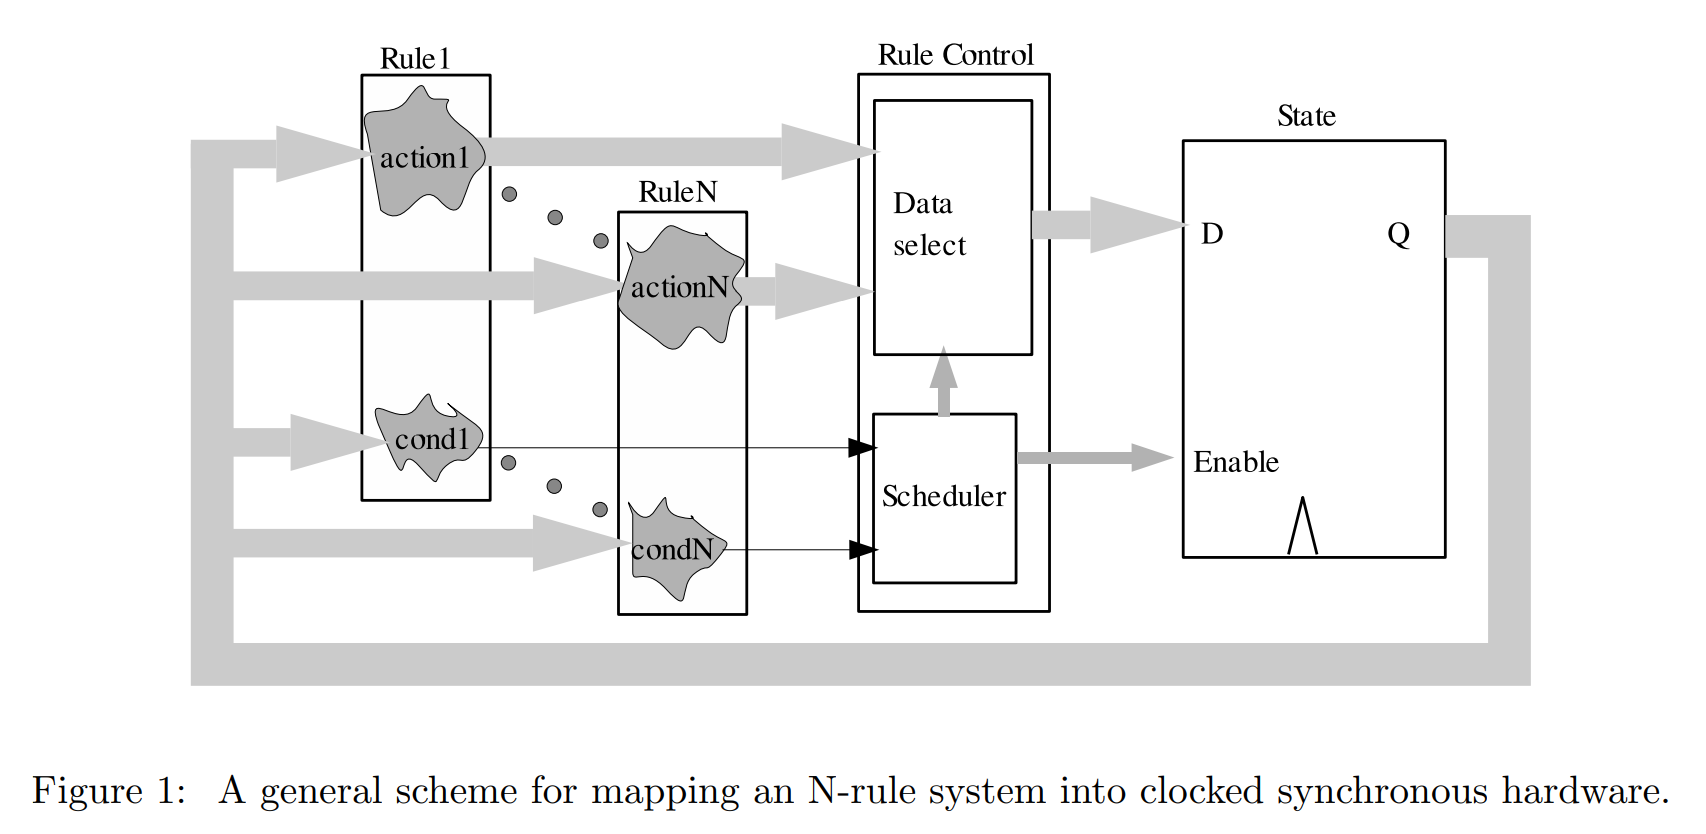
\includegraphics[]{Rulemapping.png}
    \begin{verbatim}
        
        TODO: piece of Bluespec with module using fifo and other rule explaining types of conditions.
        
    \end{verbatim}

\section{Types}
    I'm not sure how long this section need to be so I'm going to leave it for later. Idea of this section is to talk about that there are things like numeral types that are not synsesiable by definition. 

\section{Interfaces}
    In Bluespec all modules need to have interfaces. Those interfaces provide a framework for communication between modules. They are like a structs that contains only methods or sub stucts. Interfaces can be polymorphic and we will use this fact to create interfaces that allow for translation between interfaces. A common example would be polymorphic FIFO that can store any type. What's important is that this polymorphism makes it insyntesiable and it's exact type needs to be resolved before module with such type can be synthesied.
    \\
    TODO : I might add grammar for defining an interface from reference guide.  
    
\section{Methods or rather actions}
    I will fill this section later, it's going to be about distinction about Action , Value methods.
\section{Provisios}
    I will add some side note on provisos, and why handling them would require compilation of bluespec, and that I will check them via running bluespec compiler with some dummpy instantiating of module.
    
\section{Bluectl}
    Here I will explain what can be extracted from Bluectl.


\end{document}
